\begin{figure}[htb!]
	\centering
	\footnotesize

	\psfrag{1}[c][c] {$1st$}
	\psfrag{2}[c][c] {$2nd$}
	\psfrag{3}[c][c] {$3rd$}

	\psfrag{n}[c][c] {$0$}

	\psfrag{z}[c][c] {$\bm{z}$}
	\psfrag{v}[c][c] {$\bm{v}$}
	\psfrag{w}[c][c] {$\bm{w}$}

	\psfrag{e1}[c][c] {$\bm{e_{1}}$}
	\psfrag{e2}[c][c] {$\bm{e_{2}}$}

	\psfrag{al}[c][c] {$\bm{\alpha}$}

	\psfrag{Pz}[c][c] {$\bm{Pz}$}

	\psfrag{e}[c][c] {$1$}
	\psfrag{p}[c][c] {$=$}

	\psfrag{A}[c][c] {$A=$}
	\psfrag{P}[c][c] {$P_{1}A=$}
	\psfrag{Q}[c][c] {$P_{2}P_{1}A=$}
	\psfrag{M}[c][c] {$P_{3}P_{2}P_{1}A=$}

	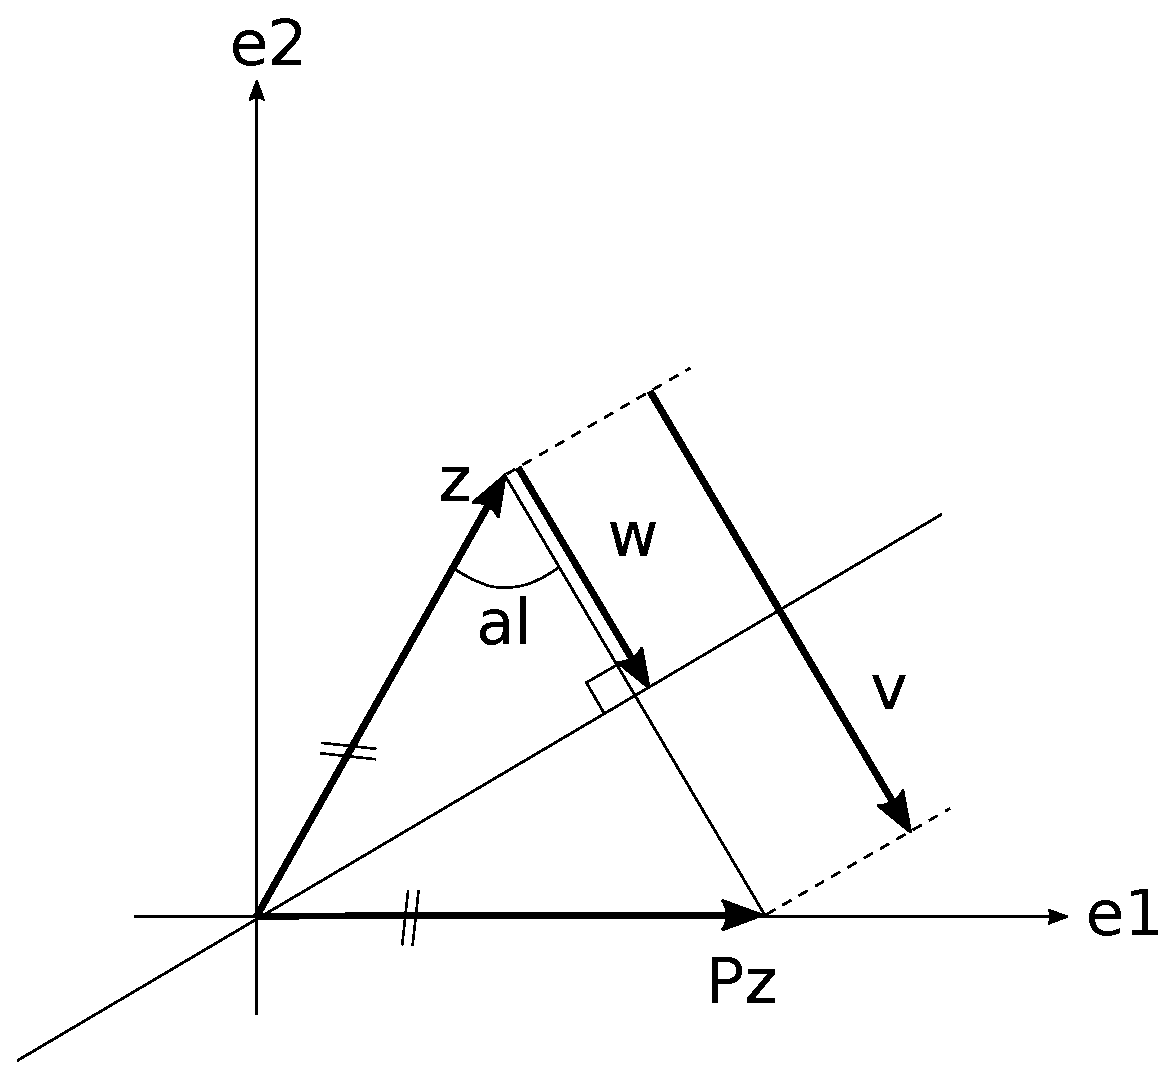
\includegraphics[width=0.99\textwidth]{householder_projection.eps}
	\caption{Consider the first column of matrix $A$.}
	\label{\LABEL}
\end{figure}